\section{Theorie}
\label{sec:Theorie}

Kehrt ein System aus einem Zustand nicht oszillierend in seinen Ruhezustand zurück, wird von einer Relaxation gesprochen.
Die zeitliche Änderung der Größe $A$ lässt sich dabei durch

\begin{equation}
    \frac{\dif A}{\dif t} = c[A(t) - A(\infty)]
    \label{eq:dAdt}
\end{equation} beschreiben, wobei $A(\infty)$ den asymptotisch erreichten Endzustand beschreibt.

Wird \eqref{eq:dAdt} nach der Zeit integriert und vereinfacht, ergibt sich

\begin{equation}
    A(t) = A(\infty) + (A(0) - A(\infty)) \,\mathrm{e}^{ct} \,.
    \label{eq:At}
\end{equation}

Damit $A(t)$ beschränkt ist, gilt $c < 0$.

Der Prozess der Relaxation lässt sich konkret am Auf- und Entladevorgang eines Kondensators über einen Widerstand beobachten, eine solche Schaltung ist in \autoref{fig:rckreis} dargestellt.

\begin{figure}[H]
    \centering
    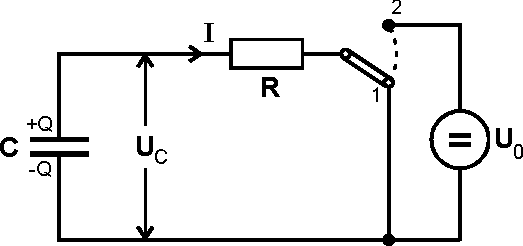
\includegraphics{figures/RC-Kreis.pdf}
    \caption{Aufladung (Schalterposition 2) und Entladung (Position 1) eines Kondensators über einen Widerstand\cite{ap08}.}
    \label{fig:rckreis}
\end{figure}

\subsubsection{Aufladevorgang}

Befindet sich der Schalter in Position 2, liegt am Kondensator die Spannung $U_0$ an.
Angenommen, zu Beginn sei der Kondensator vollständig ungeladen, gelten die Randbedingungen $Q(0) = 0$ sowie $Q(\infty) = C U_0$ mit der Kapazität $C$ des Kondensators.

Der Aufladevorgang wird dann, \eqref{eq:At} entsprechend, mit $τ := \dfrac{1}{RC}$ durch

\begin{equation*}
    Q(t) = C U_0 (1 - \text{e}^{-τ t})
    \label{eq:aufladung}
\end{equation*} beschrieben.


\subsubsection{Entladevorgang}

Ist der Kondensator nun aufgeladen, zwischen den Kondensatorplatten liegt also die Spannung $U_C = \dfrac{Q}{C}$, wird der Schalter auf Position 1 gestellt.
Nach dem ohmschen Gesetz fließt ein Strom $I_C = \dfrac{U_C}{R}$ durch den Widerstand, die Ladung am Kondensator versucht, sich auszugleichen.
Zusammen mit der in einem Zeitintervall $\dif t$ fließende Ladung
\begin{equation}
    \dif Q = -I_C \,\dif t
    \label{eq:difQ}
\end{equation} lässt sich die zeitliche Ladungsänderung auf die Form

\begin{equation*}
    \frac{\dif Q}{\dif t} = -\frac{1}{RC} Q(t)
\end{equation*} bringen.

Es gilt $Q(\infty) = 0$, da der Kondensator nach unendlicher Zeit entladen sein soll.

Die Integration nach \eqref{eq:At} liefert nun

\begin{equation*}
    Q(t) = Q(0) \text{e}^{-τ t}\,,
\end{equation*} wobei $τ$ erneut die Zeitkonstante $\dfrac{1}{RC}$ darstellt.


\subsection{Relaxation mit periodischer Anregung}

Wie in \autoref{fig:sinspann} dargestellt, wird nun ein RC-Kreis betrachtet, an dem eine Wechselspannung $U(t) = U_0 \cos(ω t)$ anliegt.

\begin{figure}[H]
    \centering
    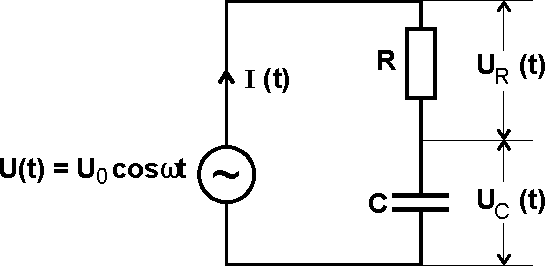
\includegraphics{figures/RC-Kreis Wechselspannung.pdf}
    \caption{RC-Kreis mit angelegter Wechselspannung $U(t)$\cite{ap08}.}
    \label{fig:sinspann}
\end{figure}

Ist die Frequenz $ω$ der Wechselspannung verschwindend gering gegen $τ$, also $ω << \frac{1}{RC}$, gilt näherungsweise $U_C(t) = U(t)$ für die Spannung $U_C$ am Kondensator.
Für höhere Frequenzen ist die Auf- bzw. Entladung des Kondensators gegenüber der Generatorspannung stark phasenverschoben.

Mit dem Ansatz

\begin{equation*}
    U_C(t) = A(ω) + \cos(ω t + \varphi(ω))
\end{equation*} und dem 2. Kirchhoffschen Gesetz

\begin{equation*}
    U(t) = U_R(t) + U_C(t)
\end{equation*} ergibt sich mithilfe von \eqref{eq:difQ}, hier

\begin{equation*}
    I(t) = \frac{\dif Q}{\dif t} = C \frac{\dif U_C}{\dif t} \,,
    \label{eq:It}
\end{equation*}
die für alle Zeitpunkte $t$ gültige Gleichung
\begin{equation}
    U_0 \cos(\omega t) = - A \omega R C  \sin(\omega t + \varphi) + A(\omega) \cos(\omega t + \varphi) \,.
    \label{eq:U_0omegagedöns}
\end{equation}

So ergibt sich z.B. für $\omega t = \frac{\pi}{2}$

\begin{equation*}
    \frac{\sin\varphi}{\cos\varphi} = \tan\varphi = -ω R C
\end{equation*} und damit 

\begin{equation}
    \varphi (ω) = \arctan(-ω R C) \,.
    \label{eq:arctan}
\end{equation}

Für niedrige Frequenzen geht $\varphi$ gegen null, für hohe Frequenzen konvergiert $\varphi$ gegen $\dfrac{\pi}{2}$.
Ist $\omega = \tau$, ist $\varphi = \dfrac{\pi}{4}$.

Für $\omega t + \varphi  = \dfrac{\pi}{2}$ folgt aus \eqref{eq:U_0omegagedöns} und \eqref{eq:arctan}

\begin{equation}
    A(\omega) = \frac{U_0}{\sqrt{1 + \omega^2 R^2 C^2}} \,.
    \label{eq:amplitudendingens}
\end{equation}

Hier ist zu erkennen, dass $A(\omega)$ für niedrige Frequenzen $\omega \rightarrow 0$ gegen $U_0$ geht, für $\omega = \dfrac{1}{RC}$ $A(\omega) = \dfrac{U_0}{\sqrt{2}}$ gilt und $A(\omega)$ für hohe Frequenzen $\omega \rightarrow \infty$ gegen null geht.
Der RC-Kreis lässt sich also als Tiefpass verwenden.

Experimentell wird die Phasenverschiebung $\varphi$ dabei \autoref{fig:phasenversch} entsprechend ermittelt.

\begin{figure}
    \centering
    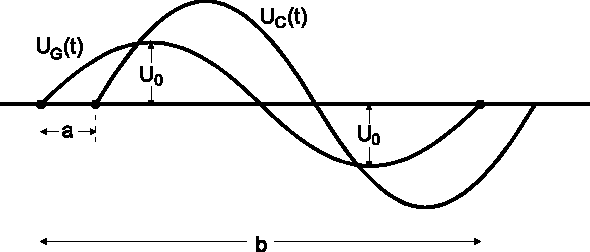
\includegraphics{figures/Phasenverschiebung.pdf}
    \caption{Messung der Phasenverschiebung zwischen der Generatorspannung und der Kondensatorspannung\cite{ap08}.}
    \label{fig:phasenversch}
\end{figure}
Es gilt

\begin{equation*}
    \varphi = 2 \pi \frac{a}{b} 
    \label{eq:phasebogen}
\end{equation*} bzw.

\begin{equation*}
    \varphi = 360 \frac{a}{b} \,.
    \label{eq:phasegrad}
\end{equation*}

%\subsection{Der RC-Kreis als Integrator}
%
%Ist $\omega >> \dfrac{1}{RC}$, ist die Spannung $U_C$ proportional zu $\int U(t) \dif t$.
%
%Mit 
%
%\begin{equation*}
%    U(t) = U_R(t) + U_C(t) = I(t) R + U_C(t)
%\end{equation*} ergibt sich mit \eqref{eq:It} und der Annahme, dass $|U_C| << |U_R|$ und $|U_C| << |U|$ 
%
%\begin{equation}
%    U(t) = RC \,\frac{\dif U_C}{\dif t}
%\end{equation}
%bzw.
%\begin{equation}
%    U_C(t) = \frac{1}{RC} \int_0^t U(t') \dif t' \,.
%    \label{eq:intkondspann}
%\end{equation}
%